%\begin{figure}[!htbp]
%    \centering
%    \caption{}
%    \includegraphics[width=0.5\textwidth]{figure_3_1.png}
%    \label{Figure 3.1}
%\end{figure}\newline

%\begin{center}
%    Truth Table 1: AND Gate Waveform
%    \begin{displaymath}
%    \begin{array}{|c c|c|}
%    In1 & In2 & In1 \land In2\\
%    \hline
%    F & F & F\\
%    F & T & F\\
%    T & F & F\\
%    T & T & T\\
%    \end{array}
%    \end{displaymath}
%\end{center}

\documentclass{article}
\usepackage{graphicx} % Required for inserting images
\usepackage{varwidth}
\usepackage{xcolor}
\usepackage{listings}

\lstdefinestyle{Verilog}{
  language=Verilog,
  basicstyle=\ttfamily\small,
  keywordstyle=\color{blue}\bfseries,
  commentstyle=\color{gray},
  stringstyle=\color{purple},
  numbers=left,
  numberstyle=\tiny,
  stepnumber=1,
  numbersep=5pt,
  tabsize=2,
  breaklines=true,
  captionpos=b,
  frame=single
}

\title{Anqa \\ \small A RISC-V Processor}
\author{Yousef Awad}
\date{February 2025}
\setcounter{secnumdepth}{0}

\begin{document}

\maketitle

\section{Opening Words}
\qquad
The objective of this processor is to implement the basic 40 instruction ISA (of which 36 are explained below) of RISC-V RV32I of which is explained in my own words, as well as explain how I went about doing it myself. I plan to make the actual processor in Vivado 2024.2 using the Verilog language.
\newpage



\tableofcontents
\newpage



\section{RV32I ISA Explained}
\subsection{Immediate-type Operations}

\subsubsection{Add Immediate}
\qquad
The 'addi' instruction is an instruction that simply adds 2 immediates (12 bits) to the register rs1, and puts it in the destination-register. The assembly is as shown below:
\begin{figure}[!htbp]
    \centering
    \begin{verbatim}
    addi destination-register,rs1,immediate-value
    \end{verbatim}
\end{figure}\newline

\subsubsection{Set Less Than Immediate}
\qquad
The 'slti' instruction is an instruction that checks if the value in register rs1 is less than the immediate-value, and if so places a value 1 in the destination-register, else it is 0. The assembly is as follows:
\begin{figure}[!htbp]
    \centering
    \begin{verbatim}
    slti destination-register,rs1,immediate-value
    \end{verbatim}
\end{figure}\newline

\subsubsection{Set Less Than Immediate Unsigned}
\qquad
The 'sltiu' instruction is an instruction that checks if the value in register rs1 is less than the immediate-value treating both values as unsigned numbers, and if so places a value 1 in the destination-register, else it is 0. The assembly is as follows:
\begin{figure}[!htbp]
    \centering
    \begin{verbatim}
    sltiu destination-register,rs1,immediate-value
    \end{verbatim}
\end{figure}\newline

\subsubsection{XOR Immediate}
\qquad
The 'xori' instruction is an instruction that performs an XOR bitwise operation on register rs1, and the signed 12-bit immediate-value, and places the result in the destination-register. The assembly is as follows:
\begin{figure}[!htbp]
    \centering
    \begin{verbatim}
    xori destination-register,rs1,immediate-value
    \end{verbatim}
\end{figure}\newline

\subsubsection{OR Immediate}
\qquad
The 'ori' instruction is an instruction that performs an OR bitwise operation on register rs1, and the signed 12-bit immediate-value, and places the result in the destination-register. The assembly is as follows:
\begin{figure}[!htbp]
    \centering
    \begin{verbatim}
    ori destination-register,rs1,immediate-value
    \end{verbatim}
\end{figure}\newline

\subsubsection{AND Immediate}
\qquad
The 'andi' instruction is an instruction that performs an AND bitwise operation on register rs1, and the signed 12-bit immediate-value, and places the result in the destination-register. This assembly is as follows:
\begin{figure}[!htbp]
    \centering
    \begin{verbatim}
    andi destination-register,rs1,immediate-value
    \end{verbatim}
\end{figure}\newline

\subsubsection{Shift Left Logical Immediate}
\qquad
The 'slli' instruction is an instruction that performs a logical left shift on the value given in register rs1 by the amount held in the last 5 bits of the immediate-value. The result is placed in the destination-register. The assembly is as follows:
\begin{figure}[!htbp]
    \centering
    \begin{verbatim}
    slli destination-register,rs1,immediate-value
    \end{verbatim}
\end{figure}\newline

\subsubsection{Shift Right Logical Immediate}
\qquad
The 'srli' instruction is an instruction that performs a logical right shift on the value given in register rs1 by the amount held in the last 5 bits of the immediate-value. The result is placed in the destination-register. The assembly is as follows:
\begin{figure}[!htbp]
    \centering
    \begin{verbatim}
    srli destination-register,rs1,immediate-value
    \end{verbatim}
\end{figure}\newline

\subsubsection{Shift Right Arithmetic Immediate}
\qquad
The 'srai' instruction is an instruction that performs an arithmetic left shift on the value given in register rs1 by the amount held in the last 5 bits of the immediate-value. The result is placed in the destination-register. The assembly is as follows:
\begin{figure}[!htbp]
    \centering
    \begin{verbatim}
    srai destination-register,rs1,immediate-value
    \end{verbatim}
\end{figure}\newline

\subsubsection{Load Byte}
\qquad
The 'lb' instruction is an instruction that loads an 8-bit value from memory (from the address taken from register rs1, with an offset of offset bytes) and sign-extends it to XLEN (32 bits in Anqa's case) and then stores it into the destination-register. The assembly is as follows:
\begin{figure}[!htbp]
    \centering
    \begin{verbatim}
    lb destination-register,offset(rs1)
    \end{verbatim}
\end{figure}\newline

\subsubsection{Load Halfword}
\qquad
The 'lh' instruction is an instruction that loads a 16-bit value from memory (from the address taken from register rs1, with an offset of offset bytes). It then sign-extends it to 32-bits and then stores it into the destination-register. The assembly is as follows:
\begin{figure}[!htbp]
    \centering
    \begin{verbatim}
    lh destination-register,offset(rs1)
    \end{verbatim}
\end{figure}\newline

\subsubsection{Load Word}
\qquad
The 'lw' instruction is an instruction that loads a 32-bit value from memory (from the address taken from register rs1, with an offset of offset bytes). It then sign-extends it to 32-bits and then stores it into the destination-register. The assembly is as follows:
\begin{figure}[!htbp]
    \centering
    \begin{verbatim}
    lw destination-register,offset(rs1)
    \end{verbatim}
\end{figure}\newline

\subsubsection{Load Byte Unsigned}
\qquad
The 'lbu' instruction is an instruction that loads an 8-bit value from memory (from the address taken from register rs1, with an offset of offset bytes). It then zero-extends it to 32-bits and then stores it into the destination-register. The assembly is as follows:
\begin{figure}[!htbp]
    \centering
    \begin{verbatim}
    lw destination-register,offset(rs1)
    \end{verbatim}
\end{figure}\newline


\subsection{Register-Register Operations}

\subsubsection{ADDition}
\qquad
The 'add' instruction is an instruction that simply adds the registers, rs1 and rs2, and puts the result in the destination-register. All arithmetic overflows are ignored. The assembly is as follows:
\begin{figure}[!htbp]
    \centering
    \begin{verbatim}
    add destination-register,rs1,rs2
    \end{verbatim}
\end{figure}\newline

\subsubsection{SUBtraction}
\qquad
The 'sub' instruction is an instruction that simply subtracts register rs2 from register rs1, and puts the result in the destination-register. All arithmetic overflows are ignored. The assembly is as follows:
\begin{figure}[!htbp]
    \centering
    \begin{verbatim}
    sub destination-register,rs1,rs2
    \end{verbatim}
\end{figure}\newline

\subsubsection{Shift Left Logical}
\qquad
The 'sll' instruction is an instruction that logical left shifts the data in register rs1 by the shift amount held in the last 5 bits of register rs2, and puts the result in the destination-register. The assembly is as follows:
\begin{figure}[!htbp]
    \centering
    \begin{verbatim}
    sll destination-register,rs1,rs2
    \end{verbatim}
\end{figure}\newline

\subsubsection{Shift Right Logical}
\qquad
The 'srl' instruction is an instruction that logical right shifts the data in register rs1 by the shift amount held in the last 5 bits of register rs2, and puts the result in the destination-register. The assembly is as follows:
\begin{figure}[!htbp]
    \centering
    \begin{verbatim}
    srl destination-register,rs1,rs2
    \end{verbatim}
\end{figure}\newline

\subsubsection{Shift Right Arithmetic}
\qquad
The 'sra' instruction is an instruction that arithmetic right shifts the data in register rs1 by the shift amount held in the last 5 bits of register rs2, and puts the result in the destination-register. The assembly is as follows:
\begin{figure}[!htbp]
    \centering
    \begin{verbatim}
    sra destination-register,rs1,rs2
    \end{verbatim}
\end{figure}\newline

\subsubsection{Set Less Than}
\qquad
The 'slt' instruction is an instruction that checks if register rs1 is less than register rs2, and if so places the value 1 in the destination-register, else it places the value 0. The assembly is as follows:
\begin{figure}[!htbp]
    \centering
    \begin{verbatim}
    slt destination-register,rs1,rs2
    \end{verbatim}
\end{figure}\newline

\subsubsection{Set Less Than Unsigned}
\qquad
The 'sltu' instruction is an instruction that checks if register rs1 is less than register rs2 treating both values in rs1 and rs2 as if they were unsigned numbers, and if so places the value 1 in the destination-register, else it places the value 0. The assembly is as follows:
\begin{figure}[!htbp]
    \centering
    \begin{verbatim}
    sltu destination-register,rs1,rs2
    \end{verbatim}
\end{figure}\newline

\subsubsection{bitwise XOR}
\qquad
The 'xor' instruction is an instruction that performs the XOR bitwise operation on registers rs1 and rs2 and places the result in the destination-register. The assembly is as follows:
\begin{figure}[!htbp]
    \centering
    \begin{verbatim}
    xor destination-register,rs1,rs2
    \end{verbatim}
\end{figure}\newline

\subsubsection{bitwise OR}
\qquad
The 'or' instruction is an instruction that performs the OR bitwise operation on registers rs1 and rs2 and places the result in the destination-register. The assembly is as follows:
\begin{figure}[!htbp]
    \centering
    \begin{verbatim}
    or destination-register,rs1,rs2
    \end{verbatim}
\end{figure}\newline

\subsubsection{bitwise AND}
\qquad
The 'and' instruction is an instruction that performs the AND bitwise operation on registers rs1 and rs2 and places the result in the destination-register. The assembly is as follows:
\begin{figure}[!htbp]
    \centering
    \begin{verbatim}
    and destination-register,rs1,rs2
    \end{verbatim}
\end{figure}\newline


\subsection{Store-type Instructions}

\subsubsection{Store Byte}
\qquad
The 'sb' instruction is an instruction that stores the least significant byte (8 bits) from the register rs2 to the memory address calculated by adding the sign-extended immediate known as offset below to the value of the register rs1. The assembly is as follows:
\begin{figure}[!htbp]
    \centering
    \begin{verbatim}
    sb rs2,offset(rs1)
    \end{verbatim}
\end{figure}\newline

\subsubsection{Store Halfword}
\qquad
The 'sh' instruction is an instruction that stores the least significant halfword (2 bytes or 16 bits) from the register rs2 to the memory address calculated by adding the sign-extended immediate known as offset below to the value of the register rs1. The assembly is as follows:
\begin{figure}[!htbp]
    \centering
    \begin{verbatim}
    sw rs2,offset(rs1)
    \end{verbatim}
\end{figure}\newline

\subsubsection{Store Word}
\qquad
The 'sh' instruction is an instruction that stores the word (4 bytes or 32 bits) from the register rs2 to the memory address calculated by adding the sign-extended immediate known as offset below to the value of the register rs1. The assembly is as follows:
\begin{figure}[!htbp]
    \centering
    \begin{verbatim}
    sh rs2,offset(rs1)
    \end{verbatim}
\end{figure}\newline


\subsection{Branch-type Instructions}

\subsubsection{Branch if EQual}
\qquad
The 'beq' instruction is an instruction that branches to the target address (that being offset), if and only if the values in registers rs1 and rs2 are equal. The assembly is as follows:
\begin{figure}[!htbp]
    \centering
    \begin{verbatim}
    beq rs1,rs2,offset
    \end{verbatim}
\end{figure}\newline

\subsubsection{Branch if Not Equal}
\qquad
The 'bne' instruction is an instruction that branches to the target address (that being offset), if and only if the values in registers rs1 and rs2 are not equal. The assembly is as follows:
\begin{figure}[!htbp]
    \centering
    \begin{verbatim}
    bne rs1,rs2,offset
    \end{verbatim}
\end{figure}\newline

\subsubsection{Branch if Less Than}
\qquad
The 'blt' instruction is an instruction that branches to the target address (that being offset), if and only if the values in registers rs1 is less than rs2. The assembly is as follows:
\begin{figure}[!htbp]
    \centering
    \begin{verbatim}
    blt rs1,rs2,offset
    \end{verbatim}
\end{figure}\newline

\subsubsection{Branch if Greater than or Equal}
\qquad
The 'bge' instruction is an instruction that branches to the target address (that being offset), if and only if the values in registers rs1 is greater than or equal to rs2. The assembly is as follows:
\begin{figure}[!htbp]
    \centering
    \begin{verbatim}
    bge rs1,rs2,offset
    \end{verbatim}
\end{figure}\newline

\subsubsection{Branch if Less That Unsigned}
\qquad
The 'bltu' instruction is an instruction that branches to the target address (that being offset), if and only if the values in registers rs1 is less than rs2, with both values being treated as if they were unsigned integers. The assembly is as follows:
\begin{figure}[!htbp]
    \centering
    \begin{verbatim}
    bltu rs1,rs2,offset
    \end{verbatim}
\end{figure}\newline

\subsubsection{Branch if Greater than or Equal Unsigned}
\qquad
The 'bgeu' instruction is an instruction that branches to the target address (that being offset), if and only if the values in registers rs1 is greater than or equal to rs2, with both values being treated as if they were unsigned integers. The assembly is as follows:
\begin{figure}[!htbp]
    \centering
    \begin{verbatim}
    bgeu rs1,rs2,offset
    \end{verbatim}
\end{figure}\newline


\subsection{Upper Immediate-type Instructions}

\subsubsection{Load Upper Immediate}
\qquad
The 'lui' instruction is an instruction that loads the 20-bit immediate value into the upper 20 bits of the destination-register, and sets the lower 12 bits to 0. The assembly is as follows:
\begin{figure}[!htbp]
    \centering
    \begin{verbatim}
    lui destination-register,immediate-value
    \end{verbatim}
\end{figure}\newline

\subsubsection{Add Upper Immediate to Program Counter}
\qquad
The 'auipc' instruction is an instruction that adds the 20-bit immediate value, shifted to the left by 12 bits, to the program counter. The assembly is as follows:
\begin{figure}[!htbp]
    \centering
    \begin{verbatim}
    auipc destination-register,immediate-value
    \end{verbatim}
\end{figure}\newline


\subsection{Jump-type Instructions}

\subsubsection{Jump And Link}
\qquad
The 'jal' instruction is an instruction that performs an unconditional (also known as immediate) jump to a target address that is calculated by adding the sign-extended immediate, shifted left by 1 bit, to the current program counter. The address of the next instruction is then saved to the destination-register. The assembly is as follows:
\begin{figure}[!htbp]
    \centering
    \begin{verbatim}
    jal destination-register,immediate-value
    \end{verbatim}
\end{figure}\newline

\subsubsection{Jump And Link Register}
\qquad
The 'jalr' instruction is an instruction that performs an unconditional (also known as immediate) jump to a target address that is calculated by adding a 12-bit sign-extended immediate, to the value in registter rs1. The least significant bit of the computed address is also cleared to ensure that it is aligned in the process. The address of the instruction following the jump (program counter + 4 bits) is then saved to the destination-register The address of the next instruction is then saved to the destination-register. The assembly is as follows:
\begin{figure}[!htbp]
    \centering
    \begin{verbatim}
    jalr destination-register,rs1,immediate-value
    \end{verbatim}
\end{figure}\newline



\newpage
\section{Part 1: The 32-bit Adder}
\qquad
First, to even design a CPU, alongside any real digital circuit, I first had to understand a basic adder, with our end goal being the 32-bit adder. However, to even understand a 32-bit adder, I first needed to understand the even simpler half adder.
\subsection{Part 1A: The Half Adder}
\qquad
A half adder is simply just, well, a device that adds 2 bits, with the following properties of which are taken from the Discrete World:
\begin{center}
    2-Bit Adder Properties
    \begin{displaymath}
    \begin{array}{|c c|c|}
    Bit1 & Bit2 & Bit1 + Bit2\\
    \hline
    0 & 0 & 0\\
    0 & 1 & 1\\
    1 & 0 & 1\\
    1 & 1 & 0\ Carry\ 1\\
    \end{array}
    \end{displaymath}
\end{center}

As you can see, when you add 2 bits, there are 3 unique cases that can happen:
\begin{enumerate}
      \item You get an output of 0.
      \item You get an output of 1.
      \item You get an output of 0 but an overflow/carry of 1.
\end{enumerate}

And now... You may be wondering, how in the world do you convert that to simple circuits using something like ANDs and ORs and XORs and NOTs??? Well, let's think, what does the table itself look like? It looks like a gate that is ONLY true when either Bit1 or Bit2 is enabled...
But what of the carry? Well, when is that enabled? It's only on when BOTH Bit1 and Bit2 are on, therefore isn't it literally just an AND gate? Therefore, wouldn't the circuit look something like this?
\begin{figure}[!htbp]
    \centering
    \caption{The Basic Half Adder Schematic as described in the paragraph above}
    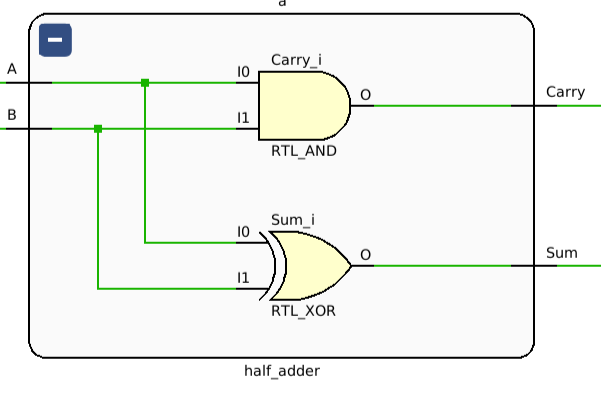
\includegraphics[width=0.75\textwidth]{pictures/part1/basic_half_adder.png}
    \label{Basic 2-Bit Adder}
\end{figure}

And of which, at least when coded in Verilog, would look like this:
\begin{lstlisting}[caption={Half Adder Verilog Code}, label={Half Adder Verilog}, style=Verilog]
module half_adder(
        input Bit1, Bit2,
        output Sum, Carry
    );
    
    assign Sum = Bit1 ^ Bit2; // ^ is XOR
    assign Carry = Bit1 & Bit2; // & is AND
    
endmodule
\end{lstlisting}

\subsection{Part 1B: The Full Adder}
\qquad
Now, we got a problem... What if we have a carry in from another adder, or say just a previous bit addition? Well, we could just chain the half adders! And get the following schematic, and Verilog code!
\begin{figure}[!htbp]
    \centering
    \caption{A Full Adder as described in the paragraph above}
    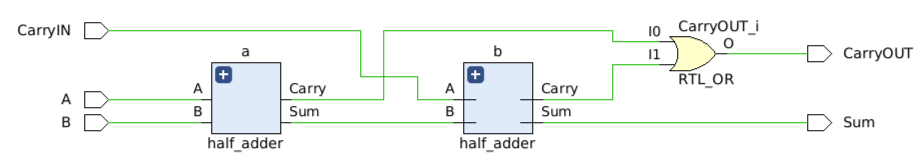
\includegraphics[width=0.75\textwidth]{pictures/part1/full_adder.png}
    \label{Full Adder}
\end{figure}
\begin{lstlisting}[caption={Full Adder Verilog Code}, label={Full Adder Verilog}, style=Verilog]
module full_adder(
        input A, B, CarryIN,
        output Sum, CarryOUT
    );
    
    wire carry1, carry2, sum1;
    
    half_adder a(.Bit1(A), .Bit2(B), .Carry(carry1), .Sum(sum1));
    half_adder b(.Bit1(CarryIN), .Bit2(sum1), .Carry(carry2), .Sum(Sum));
    
    assign CarryOUT = carry1 | carry2; 
    
endmodule
\end{lstlisting}

\subsection{Part 1C: Chaining Adders Together}
\qquad And now we get to a fun part, a part where we get to chain the adders together into 2 bit adders, and 4 bit adders, etc etc until we get to a 32 bit adder. To do this, though, I shall be taking it in the approach that, for now, it will be made up of two 16 bit adders, of which is made up of two 8 bit adders, and so on. I'll only be showing the code for the 2 bit adder though, as after that it is the same structure with different names.\\

Therefore, how in the world do we chain the two bits together into a result that lets you add two 2 bit numbers together? Well, let's think about it, we have 2 bits in an array, number 1, of which is two bits long, and number 2, of which is also two bits long. Woouldn't we have to add the least significant bit first (of which is, if you didn't know, the right-most bit), and then output the result to the output bit, as well as the carry out to the carry in of the bit to the left of it? So, let's try that out in with the following verilog code, and guess what it's correct:\\
\begin{lstlisting}[caption={2 Bit Adder Verilog Code}, label={2 Bit Adder Verilog}, style=Verilog]
module two_bit_adder(
        input[1:0] A, B,
        input CarryIN,
        output[1:0] Sum,
        output CarryOUT
    );
    
    wire carry;
    
    full_adder a(.A(A[0]), .B(B[0]), .CarryIN(CarryIN), .CarryOUT(carry), .Sum(Sum[0]));
    full_adder b(.A(A[1]), .B(B[1]), .CarryIN(carry), .CarryOUT(CarryOUT), .Sum(Sum[1]));
    
endmodule
\end{lstlisting}

Of which generates the following schematic:
\begin{figure}[!htbp]
    \centering
    \caption{2 Bit Adder as designed above}
    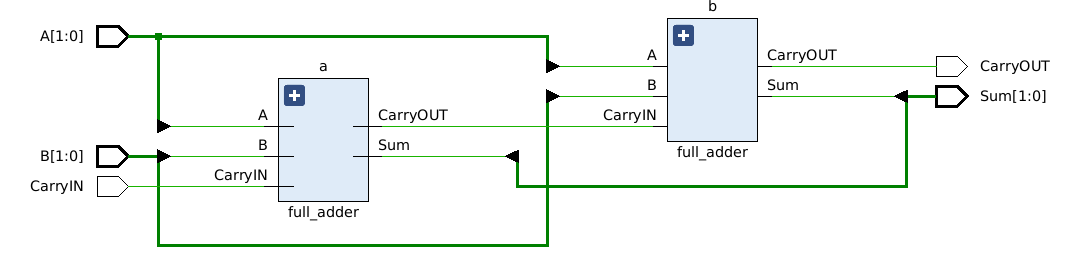
\includegraphics[width=0.75\textwidth]{pictures/part1/two_bit_adder.png}
    \label{2 Bit Adder}
\end{figure}\newpage

And now, to just spoil the fun for you, I'll just tell you that, guess what, it's the exact same thing for every addition to it, from 4 bits to 32 bits to even 128 bits if you wanted. And so, I'll just show you the 32 bit encapsulation, and to find the submodules in it head to the code proper in sources...
\begin{lstlisting}[caption={32 Bit Adder Verilog Code}, label={32 Bit Adder Verilog}, style=Verilog]
module thirtytwo_bit_adder(
        input[31:0] A, B,
        input CarryIN,
        output[31:0] Sum,
        output CarryOUT
    );
    
    wire carry;
    
    sixteen_bit_adder a(.A(A[15:0]), .B(B[15:0]), .CarryIN(CarryIN), .CarryOUT(carry), .Sum(Sum[15:0]));
    sixteen_bit_adder b(.A(A[31:16]), .B(B[31:16]), .CarryIN(carry), .CarryOUT(CarryOUT), .Sum(Sum[31:16]));
    
endmodule
\end{lstlisting}

Of which generates the following schematic:
\begin{figure}[!htbp]
    \centering
    \caption{32 Bit Adder as designed above}
    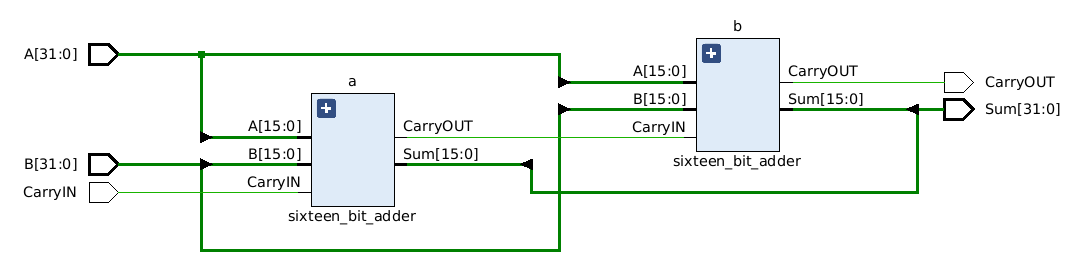
\includegraphics[width=0.75\textwidth]{pictures/part1/thirtytwo_bit_adder.png}
    \label{32 Bit Adder}
\end{figure}



\newpage
\section{Important Definitions}

\subsection{Arithmetic Shifting}
\qquad
This is a bitwise operation that, like logical shifting, moves all of the bits of a binary of bit-length X, left or right by a specificied number of positions/bits. Unlike logical shifting, however, you would preserve the sign of the number and therefore when shifting a negative number would fill with 1s or if positive would be 0s.

\subsection{Immediate Values}
\qquad
An immediate value is a constant that is embeded directly into an instruction. This means that it is not stored in a register or memory location, and therefore does not need to access anything before using the value, making the value usable immediately after its declaration.

\subsection{Logical Shifting}
\qquad
This is a bitwise operation that moves all of the bits of the binary number of bit-length X, left or right by a specificied number of positions/bits. The vacant bits, if any are created, are subsequently filled with 0s.

\subsection{Program Counter (PC)}
\qquad
The program counter is a special register that holds the memory address of the next instruction that is going to be executed.

\subsection{Sign Extension}
\qquad
This is the process of increasing the bit-width of a binary number while preserving its value and sign from the original. To do this, you duplicate the most significant bit into the new empty bits that are higher order than the original bit-width.

\subsection{Zero Extension}
\qquad
This is the process of increasing the bit-width of a binary number but, unlike sign extensions, is only used for unsigned binary numbers and only simply adds 0s to the higher order bits, therefore only preserving the original value.


\end{document}
